\documentclass[../main.tex]{subfiles}

\graphicspath{{\subfix{../images/}}}

\begin{document}

\section{Task 5}

Create a new function called \texttt{multiMatrixHard} that computes the matrix product of the expression $P = A \times B^T$ but use the new IP core \texttt{matrix\_ip} to perform part of the matrix multiplication.

\vspace{10pt}

Display result P and the execution time (in clock ticks) of the function \texttt{multiMatrixHard} in the USB UART window and compare it to \texttt{multiMatrixSoft}. The ARM processor (PS) runs at 650 MHz and the hardware matrix multiplication (PL) is clocking at 100 MHz. The timer is running at half of the PS clock (325 MHz). Evaluate the computation speed of software vs. hardware implementation based on measured execution time and clock speeds.

\subsection*{Solution}

We write an entire row of matrix A and B to slave registers 0 and 1, respectively, of the matrix IP. The IP core then computes the dot product of the two rows and writes the result to slave register 2 which is then read back into matrix P. This process is repeated for all rows of matrix A and B.

\begin{myminted}{matrixMultiplication.c - multiplyMatricesHard()}
void multiplyMatricesHard(vectorArray matrixA, vectorArray matrixB, vectorArray matrixP)
{
    for (int row = 0; row < MATRIX_SIZE; row++) {
        for (int col = 0; col < MATRIX_SIZE; col++) {
            Xil_Out32(XPAR_MATRIX_IP_S00_AXI_BASEADDR + MATRIX_IP_S_AXI_SLV_REG0_OFFSET, matrixA[row].vect);
            Xil_Out32(XPAR_MATRIX_IP_S00_AXI_BASEADDR + MATRIX_IP_S_AXI_SLV_REG1_OFFSET, matrixB[col].vect);
            matrixP[row].comp[col] = Xil_In32(XPAR_MATRIX_IP_S00_AXI_BASEADDR + MATRIX_IP_S_AXI_SLV_REG2_OFFSET);
        }
    }
}
\end{myminted}

The main switch-case statement is expanded to include an example showcasing hard matrix multiplication, selected by the user by entering '4' in the terminal.

\begin{myminted}{main.c - Hard Matrix Multiplication Switch Case}
case '4':
    xil_printf("\r\nStarting Program 4.");
    xil_printf("\r\nHard Matrix Multiplication.");
    TimerStop(&TimerInstance);
    TimerFunctionPtr = NULL;
    TimerLoad(&TimerInstance, 1000*MILLISECOND);
    TimerStart(&TimerInstance);
    matrix_hard();
    break;
\end{myminted}

\newpage

The function \texttt{matrix\_hard()} closely resembles the \texttt{matrix\_soft()} function, but instead of calling \texttt{multiplyMatricesSoft()} it calls \texttt{multiplyMatricesHard()}.

\begin{myminted}{main.c - matrix\_hard()}
void matrix_hard()
{
	vectorArray matrixA, matrixB, matrixP;
	u32 start, end;

	setInputMatrices(matrixA, matrixB);

	xil_printf("\r\n\nMatrix A:\r\n");
	displayMatrix(matrixA);

	xil_printf("\r\n\nMatrix B:\r\n");
	displayMatrix(matrixB);

	start = XScuTimer_GetCounterValue(&TimerInstance);
	multiplyMatricesHard(matrixA, matrixB, matrixP);
	end = XScuTimer_GetCounterValue(&TimerInstance);

	xil_printf("\r\n\nMatrix P (Result of multiplication):\r\n");
	displayMatrix(matrixP);

	/* Subtract 'end' from 'start' since XScuTimer is down counting */
	xil_printf("Clock cycles: %llu\n", 2 * (start - end));
}
\end{myminted}

\begin{figure}[h]
    \centering
    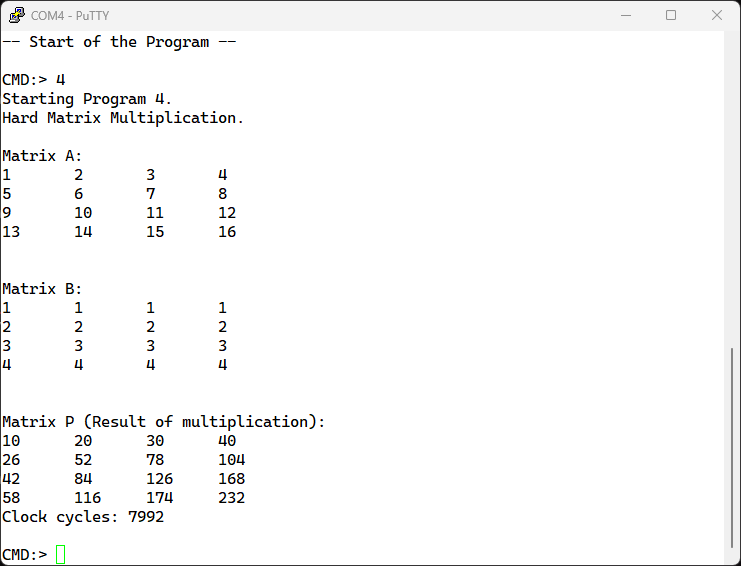
\includegraphics[width=1\textwidth]{task5_putty.png}
\end{figure}

\newpage

We see that it takes approximately 8000 clock cycles to compute the matrix product using the hardware IP core. This is \textit{worse} than the software implementation. 

\end{document}